%!TEX root = ../../super_main.tex

\section{Launcher}

Our group opted for, and got assigned to, improving the \giraf-\launcher application during a meeting between representatives of the GUI project area groups.\\

The \giraf-\launcher is specialized Android launcher application which can be used to populate the home screen of an Android device. Most Android devices come bundled with a default launcher for their home screen and most users never think to replace it. An Android launcher is the main entry point, for users, to the graphical user interface for Android. Android launchers are used to make other installed applications available to the user, usually through a grid of application icons, and to present Android Widgets. The intended purpose of the \giraf-\launcher, besides the functionality of a regular launcher, is to give the user a single entrance to the \giraf software suite and to give the illusion of using the \giraf-system and not Android. A screenshot of the \androidinline{HomeActivity} of the launcher can be seen in \figref{fig:initial_launcher}\\

The \launcher project also contains the login and authentication part of the \giraf suite, which a user has to pass through before being able to use the application. The authentication system is being developed by another SW6 group in the first sprint, and will therefore not be considered in this part of the report. 

\begin{figure}[!htbp]
	\centering
	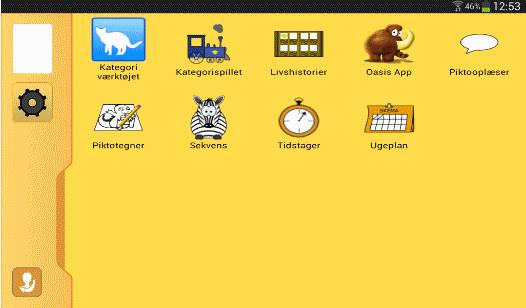
\includegraphics[width=\textwidth]{sprint_one/initial_launcher}
	\caption{Initial Launcher}
	\label{fig:initial_launcher}
\end{figure}
